\chapter{Design del sistema}

\section{Introduzione}
In questo documento mostreremo delle soluzioni concrete per il modello di analisi effettuato nel documento di \docref{cha:analisi}, aggiungeremo quindi il \emph{come} al \emph{cosa}. Mostreremo quindi una specifica architetture del sistema e aggiungeremo il necessario per rendere possibile l'implementazione dei requisiti formalizzati nel documento di \docref{cha:specifica_requisiti}.

\section{Architettura del sistema}
Per realizzare il sistema finora descritto utilizzeremo il \gls{cms} commerciale WordPress, scelto in quanto dispone di una grande quantità di plugin necessari per soddisfare tutte le funzionalità necessarie. Questo sarà installato nel server e si occuperà della comunicazione con i fruitori del servizio e con il database.

\subsection{Architettura fisica}
L'architettura fisica del sistema è mostrata dalla seguente figura:
\begin{center}
   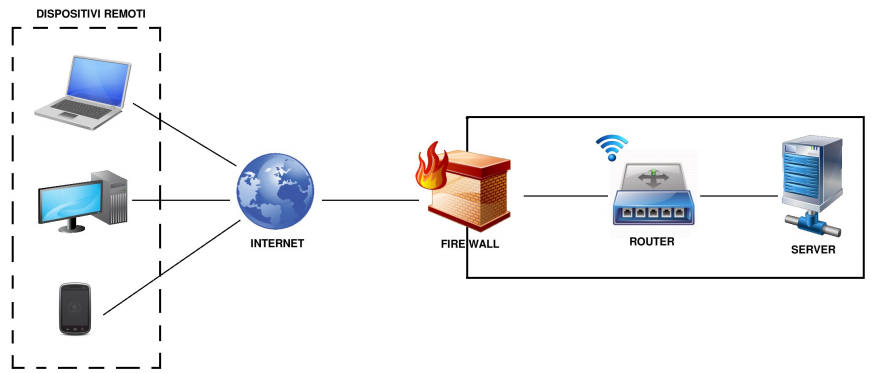
\includegraphics[width=\textwidth]{assets/architetturaFisica}
\end{center}


\subsection{Architettura software}
L'architettura software del sistema è mostrata dalla seguente figura:
\begin{center}
   \includegraphics[width=\textwidth]{assets/architetturaSoftware}
\end{center}























